\documentclass[11pt]{article} 
\usepackage[french]{babel}
\usepackage[T1]{fontenc}
\usepackage[lmargin=1in,rmargin=1in,tmargin=1in,bmargin=1in]{geometry}
\usepackage{amsfonts,amsmath, amssymb,array}
\usepackage{graphicx}
\usepackage{titlesec}
\usepackage{filecontents} 
\usepackage{amsmath}


\titleclass{\subsubsubsection}{straight}[\subsection]

\newcounter{subsubsubsection}[subsubsection]
\renewcommand\thesubsubsubsection{\thesubsubsection.\arabic{subsubsubsection}}


\titleformat{\subsubsubsection}
  {\normalfont\normalsize\bfseries}{\thesubsubsubsection}{1em}{}
\titlespacing*{\subsubsubsection}
{0pt}{3.25ex plus 1ex minus .2ex}{1.5ex plus .2ex}

\titleformat{\paragraph}
  {\normalfont\normalsize\bfseries}{\theparagraph}{1em}{}
\titlespacing*{\paragraph}
{0pt}{3.25ex plus 1ex minus .2ex}{1.5ex plus .2ex}

\makeatletter
\renewcommand\subparagraph{\@startsection{subparagraph}{6}{\parindent}%
  {3.25ex \@plus1ex \@minus .2ex}%
  {-1em}%
  {\normalfont\normalsize\bfseries}}
\def\toclevel@subsubsubsection{4}
\def\toclevel@paragraph{5}
\def\toclevel@paragraph{6}
\def\l@subsubsubsection{\@dottedtocline{4}{7em}{4em}}
\def\l@paragraph{\@dottedtocline{5}{10em}{5em}}
\def\l@subparagraph{\@dottedtocline{6}{14em}{6em}}
\makeatother
\newcommand{\HRule}{\rule{\linewidth}{0.5mm}}

\setcounter{secnumdepth}{4}
\setcounter{tocdepth}{4}

%\input{mymathsym}
%% symboles mathématiques
\newcommand{\E}{\mathbb{E}}
\newcommand{\Pro}{\mathbb{P}}
\newcommand{\Rset}{\mathbb{R}}
\newcommand{\Nset}{\mathbb{N}}	

\newcommand{\cB}{\mathcal{B}}
\newcommand{\cL}{\mathcal{L}}
\newcommand{\cN}{\mathcal{N}}



\newcommand{\bsX}{\boldsymbol{X}}
\newcommand{\bsx}{\boldsymbol{x}}
\newcommand{\bsy}{\boldsymbol{y}}
\newcommand{\bsp}{\boldsymbol{p}}
\newcommand{\bsz}{\boldsymbol{z}}
\newcommand{\bsk}{\boldsymbol{k}}
\newcommand{\bst}{\boldsymbol{t}}
\newcommand{\bsA}{\boldsymbol{A}}
\newcommand{\bsh}{\boldsymbol{h}}
\newcommand{\bsW}{\boldsymbol{W}}
\newcommand{\bsI}{\boldsymbol{I}}
\newcommand{\bse}{\boldsymbol{e}}


\newcommand{\ciz}{\textit{z}}
\newcommand{\cif}{\textit{f}}
\newcommand{\ciy}{\textit{y}}
\newcommand{\cih}{\textit{h}}
\newcommand{\cil}{\textit{l}}
\newcommand{\cik}{\textit{k}}
\newcommand{\ciQ}{\textit{Q}}
\newcommand{\cia}{\textit{a}}
\newcommand{\cib}{\textit{b}}
\newcommand{\cir}{\textit{r}}
\newcommand{\cii}{\textit{i}}



\newcommand{\sumn}{\sum_{i=1}^{n}}
\newcommand{\sumK}{\sum_{k=1}^{K}}
\newcommand{\sumR}{\sum_{r=1}^{R}}
\newcommand{\sumttn}{\sum_{i=2}^{n}}
\newcommand{\sumtn}{\sum_{i=1}^{n}}
\newcommand{\sumlK}{\sum_{l=1}^{K}}


\newcommand{\bX}{\mathbf{X}}
\newcommand{\bY}{\mathbf{Y}}
\newcommand{\bZ}{\mathbf{Z}}
\newcommand{\bK}{\mathbf{K}}
\newcommand{\bA}{\mathbf{A}}
\newcommand{\bB}{\mathbf{B}}


\newcommand{\bstheta}{\boldsymbol{\theta}}
\newcommand{\bsPsi}{\boldsymbol{\Psi}}
\newcommand{\bsbeta}{\boldsymbol{\beta}}
\newcommand{\betakT}{\boldsymbol{\beta}_{k}^{T}}
\newcommand{\betaT}{\boldsymbol{\beta}^{T}}



\begin{document}
\begin{titlepage}
\begin{center}
	\begin{figure}
		\begin{minipage}[c]{.46\linewidth}
      			\begin{flushleft}		
			
\includegraphics[height=3cm]{unicaen.png}
	  		\end{flushleft}
    		\end{minipage}
		
    \end{figure}
    \textsc{\LARGE Université de Caen Normandie}\\[1cm]

\begin{figure}[h]
\begin{center}
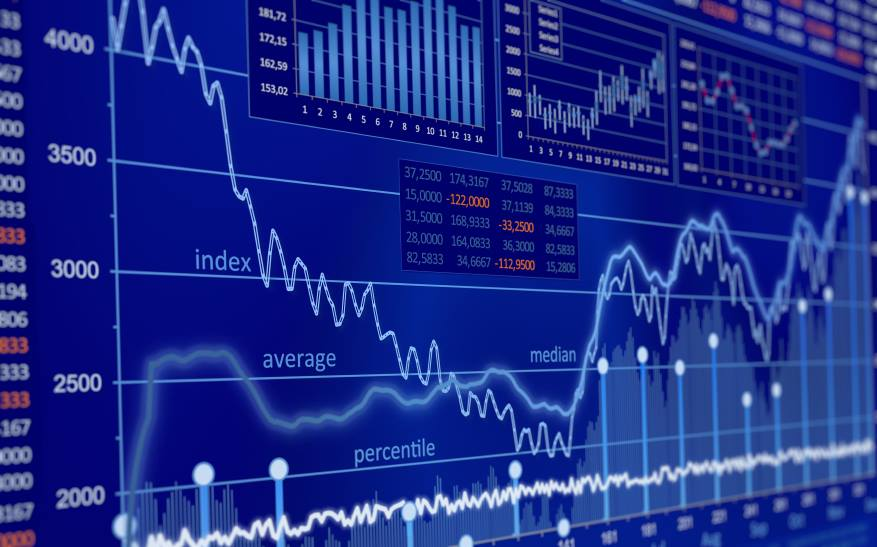
\includegraphics[height=5cm]{img.jpg}
\end{center}
\end{figure}
    
    % Title
    \HRule \\[0.4cm]
    { \huge \bfseries Régression à l'aide du modèle de Markov caché }

\HRule \\[6.5cm]


    % Author and supervisor
    
    \begin{minipage}{0.4\textwidth}
      \begin{flushleft} \large
        \emph{Auteurs :}S.Blin A.Bourjal C.Champarou\\
        \emph{M2 Statistiques Appliquées et Analyse Décisionnelle}
      \end{flushleft}
    \end{minipage}
    \begin{minipage}{0.4\textwidth}
      \begin{flushright} \large
        \emph{Tuteur projet :} M. \textsc{F.Chamroukhi}\\
      \end{flushright}
    \end{minipage}

    \vfill

    % Bottom of the page
    Année universitaire 2018-2019


\end{center}
\end{titlepage}




\newpage
\tableofcontents
\newpage
\section*{Modèle}

Dans la régression de modèle de Markov cachée (HMMR), chaque série temporelle est représentée par une séquence de variables univariées observées. $(\bsy_{1},\bsy_{2},\ldots,\bsy_{n})$ où l'observation $\bsy$ à l'heure $\bst$ est supposée être généré par le modèle de régression suivant: 

\begin{equation}
\bsy_{i} = \beta \bst_{i} + \sigma \epsilon_{i} \ ; \ \epsilon_{i} \sim \cN(0,1), \ ( i = 1,\ldots,n)
\end{equation}

Ainsi le modèle précédent peut être réécris sous la forme matricielle suivante : \\

\begin{equation}
\bsy_{i} = \bB \bst_{i} + \bse_{i} \  ; \  \bse_{i} \sim \cN(0,\sigma^{2}), \ (i=1,\ldots,n)
\end{equation}

où $\bsy_{i}$ est la ith observation de la séries temporelle dans $\Rset$



\section{Paramètre}

Le modèle Multiple HMMR est donc entièrement paramétré par le vecteur de paramètre $\bsPsi =(\pi,\bA,\bB,\sigma_{1}^{2}, \ldots,  ,\sigma_{K}^{2})$. La sous-section suivante décrit la technique d’estimation des paramètres en maximisant la vraisemblance des données observées au moyen de l’algorithme Expectation-Maximization (EM). 


\section{Estimation}

Soit $\bsPsi$ : le vecteur de paramètre du modèle à estimé. \\
 

\subsection{Estimation par Maximum de vraisemblance}

Le vecteur de paramètre $\bsPsi$ est estimé en utilisant la méthode bien connue du maximum de vraisemblance grâce à ses propriétés attractives très connues de cohérence, de normalité asymptotique et d’efficacité. En effet, dans nos expériences, un nombre considérable de points de données est acquis au fil du temps, ce qui rend la taille de l'échantillon appropriée pour tirer parti des propriétés limites de l'estimateur du maximum de vraisemblance. Le log-vraisemblance à maximiser dans ce cas est écrit comme suit: 


\begin{equation}
\cL(\bsPsi) = \text{log} \ \bsp(\bsy_{1},\ldots,\bsy_{n} ; \bsPsi) \
\end{equation}

\begin{equation}
\cL (\bsPsi) =  log \sum_{z_{1},\ldots,z_{n}} \bsp(\ciz_{1},\pi) \prod_{i=2}^{n}\bsp(\ciz_{i}|\ciz_{i-1};\bA) \prod_{t=1}^{n}\bsp(\bsy_{i};\bsPsi).
\end{equation}



Cette log-vraisemblance est difficile à maximiser directement ,d'ou l'utilisation d'un algorithme  performent qui est nommé l' algorithme d' expectation maximisation (EM).\\


\subsection{Estimation  par l'ALgorithme EM}


L'algorithme espérance-maximisation (en anglais expectation-maximization algorithm, souvent abrégé EM) est un algorithme itératif qui permet de trouver les paramètres du maximum de vraisemblance d'un modèle probabiliste lorsque ce dernier dépend de variables latentes non observables. De nombreuses variantes ont par la suite été proposées, formant une classe entière d'algorithmes. \\



\subsubsection{Etape E}

L'étape E calcul une estimation de la log-vraisemblance des données complètes : \\


\begin{equation}
\ciQ (\bsPsi,\bsPsi^{(q)}) = \E \big[ \ \text{log} \ \bsp( \bY, \bsz | \bst ; \bsPsi) | \bY, \bst ; \bsPsi \big]
\end{equation}


Il est facile de montrer que l'etape E n'a besoin, seulement, de calculer les probabilités à postériori de $\epsilon_{ilk}^{(q)}$ et $\tau_{ik}^{(q)}$. Ces dernier calculer par les récursions du forward-backward. \\



\paragraph{Forward-Backward}

Le processus du forward calcul recursivement les probabilités :\\

\begin{equation}
\tau_{ik}^{(q)}=\bsp( \ciz_{i} = \bsk | \bY,\bst, \bsPsi^{(q)}) 
\end{equation}

Les probabilités à postériori jointes de l'état $\bsk$ à un temps $\cii$ et l'état $\cil$ à l'état $\cii-1$ donne la sequence d'observations : \\

\begin{equation}
\epsilon_{ilk}^{(q)} = \bsp (\ciz_{i} = \bsk, \ciz_{i-1} = \cil | \bY, \bst ; \bsPsi^{(q)})
\end{equation}


\subsubsection{Etape M}

Dans cette étape, la valeur du paramètre est mise à jour en calculant le paramètre qui maximise l'attente conditionnelle par rapport à $\bsPsi$ . On peut montrer que cette maximisation conduit aux règles de mise à jour suivantes. Les mises à jour des paramètres gouvernant la chaîne de Markov cachée sont ceux d’un HMM standard et sont donnés :  


\begin{equation}
\pi_{k}^{(q+1)}=\tau_{1k}^{(q)}
\end{equation}

\begin{equation}
\bA_{lk}^{(q+1)}= \frac{\sumttn \epsilon_{ilk}^{(q)}}{\sumttn \tau_{ik}^{(q)}}
\end{equation}

\begin{equation}
\bB_{k}^{(q+1)}= ( \bsX^{T} \bsW_{k}^{(q)} \bsX)^{-1} \bsX^{T} \bsW_{k}^{(q)} \bY
\end{equation}

\begin{equation}
\sigma_{k}^{2(q+1)}= \frac{1}{\sumn \tau_{ik}^{(q)}} (\bY - \bX \bB_{k}^{(q+1)})^{T} \bsW_{k}^{(q)}( \bY - \bX \bB_{k}^{(q+1)})
\end{equation}

\newpage
\section{Application}

Dans cette section, nous présenterons l'utilisation de la régression à l'aide du modèle de Markov sur des données simulées. Celle-ci sont représenté sur le graphe suivant : \\

\begin{figure}[h]
\begin{center}
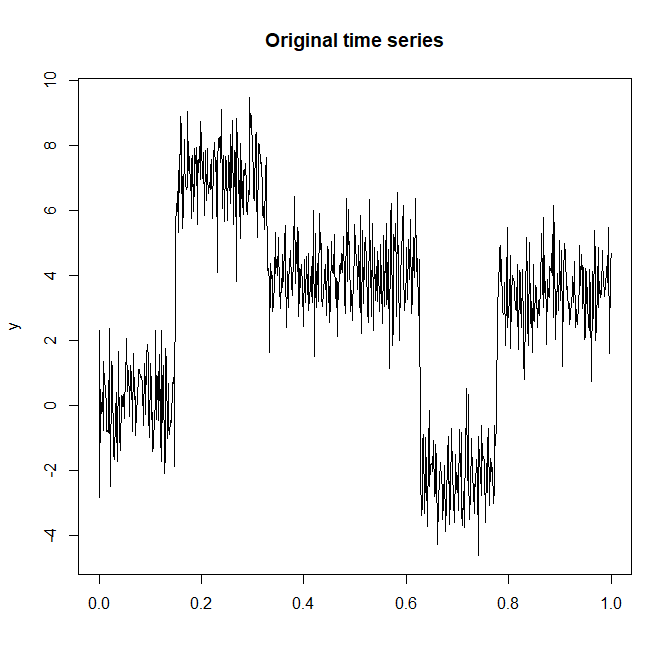
\includegraphics[height=8cm]{data.png}
\end{center}
\end{figure}

Nous pouvons constater que le graphe peut être séparé en 5 parties disctinctes. Nous supposons donc que cela réprensentera 5 états différents dans l'exemple que nous étudions sur ces données simulées. Afin de confirmer nos conjectures, nous utilisons le Bayesian information criterion (BIC) afin de déterminer le nombre de classes et l'odre de notre regression polynomiale. \\


\begin{figure}[h]
\begin{center}
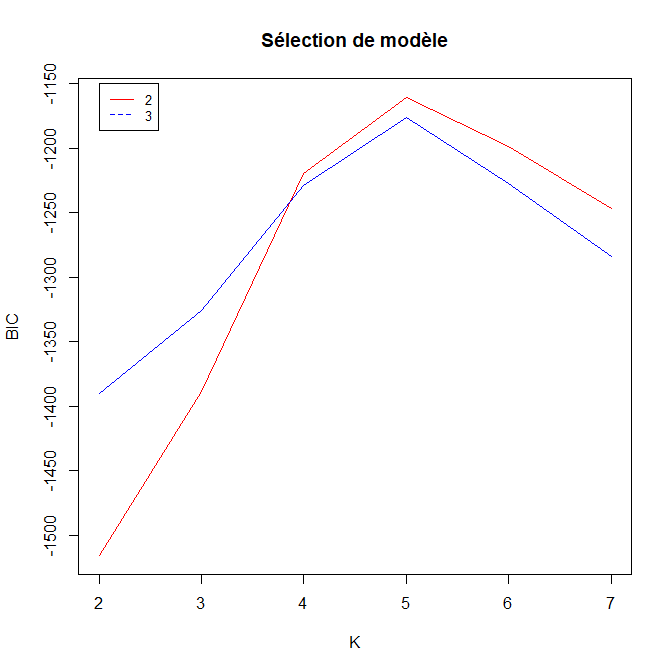
\includegraphics[height=8cm]{bic.png}
\end{center}
\end{figure}

Dans ce graphique, on peut constater qu'il y a un pic en $\bK$=5 pour les 2 lignes. Ce pic confirme notre hypothèse faite précédemment sur le nombre de classe. On choisira l'ordre de notre regression polynomiale égale à 2 car c'est la valeur la plus élevée pour $\bK$=5.\\

Pour la suite de notre étude, on choisit $\bK$=5, $\bsp$=2 et l'hétéroscédaticité pour nos données. On utilisera l'algorithme EM pour estimer nos paramètre.\\

\begin{figure}[h]
\begin{center}
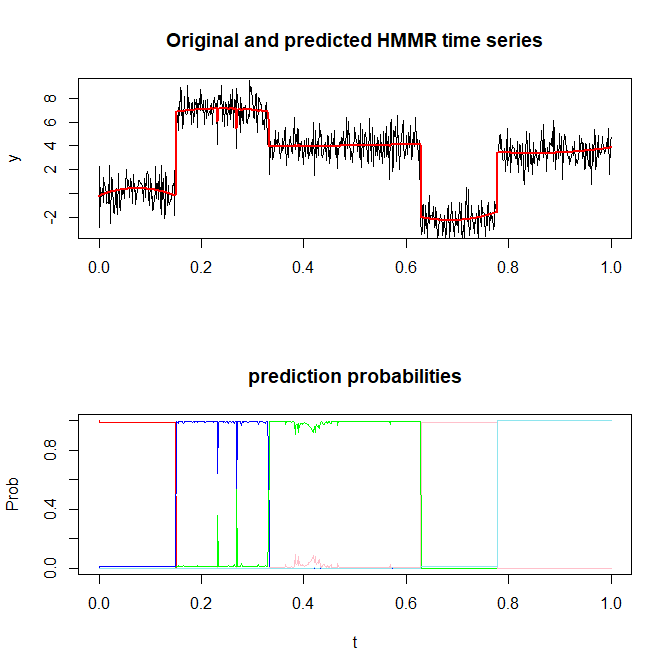
\includegraphics[height=8cm]{prediction.png}
\end{center}
\end{figure}

La prédiction nous donne le graphique ci-dessus. Grâce à cela nous avons donc découpé le graphique en fonction du nombre de classe que nous disposions nous donnant le graphique suivant : \\

\begin{figure}[h]
\begin{center}
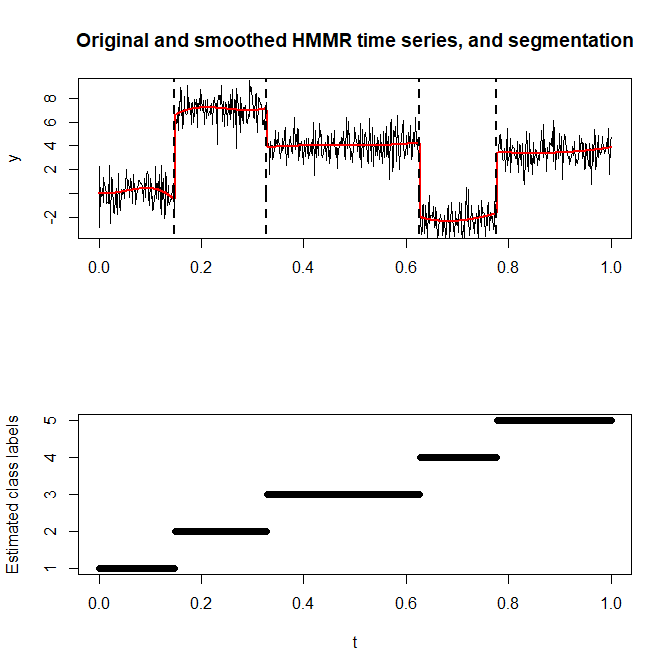
\includegraphics[height=8cm]{separationclasse.png}
\end{center}
\end{figure}

Enfin, nous avons estimé les différents segments de tel manière à ce que chaque segment aie une fonction polynomiale qui l'ajuste

\begin{figure}[h]
\begin{center}
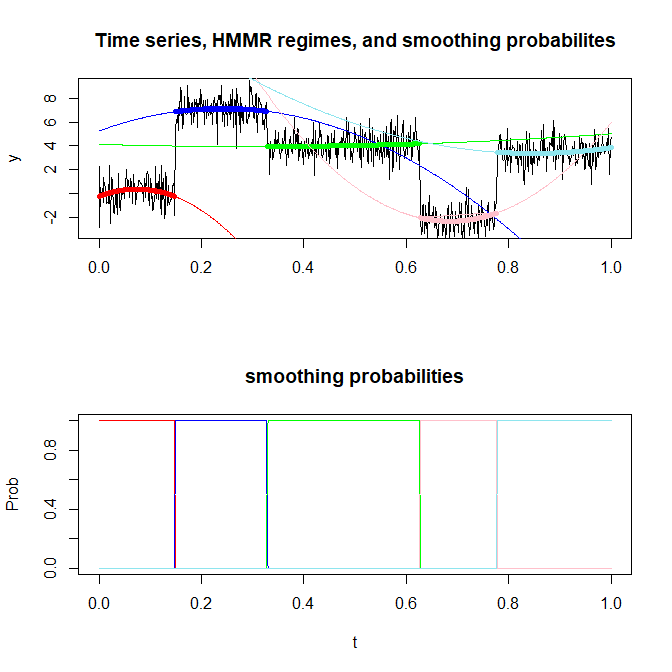
\includegraphics[height=8cm]{lissage.png}
\end{center}
\end{figure}





\end{document}